\documentclass[11pt]{article}
\usepackage[utf8]{inputenc}
\usepackage[T1]{fontenc}
\usepackage{geometry}
\geometry{a4paper, margin=1in}
\usepackage{booktabs}
\usepackage{hyperref}
\usepackage{amsmath, amssymb}
\usepackage{graphicx}
\usepackage{caption}
\usepackage{subcaption}
\usepackage{xcolor}
\usepackage{float}
\usepackage{algorithm}
\usepackage{algorithmicx}
\usepackage{algpseudocode}
\usepackage{tikz}
\usetikzlibrary{decorations.pathreplacing, positioning}

\title{The Li-Chao tree: An Alternative Approach to Dynamic Maintenance of the Lower Envelope}
\author{Li Chao}
\date{\today}

\begin{document}

\maketitle

\begin{abstract}
The Li-Chao tree (LICT) is a specialized segment tree variant designed for the dynamic maintenance of a lower envelope of lines or line segments. It provides an alternative to the traditional Convex Hull Trick (CHT), particularly in scenarios requiring online insertions of lines with arbitrary slopes and queries at arbitrary coordinates. This report provides a formal description of the algorithm, its geometric intuition, and a performance comparison across various implementation variants.
\end{abstract}

\section{Introduction}
The problem of maintaining the lower envelope of a set of linear functions $f_i(x) = k_i x + b_i$ is fundamental in computational geometry and has extensive applications in competitive programming, particularly for optimizing dynamic programming transitions. While the Convex Hull Trick (CHT) is a well-established solution, its dynamic variant often involves complex balanced binary search trees or specialized data structures to handle non-monotonic slopes and queries.

The Li-Chao tree, introduced by Li Chao in 2012, offers a conceptually simpler approach based on the segment tree structure. By storing lines directly in the nodes of a range tree, it achieves $O(\log C)$ time complexity for both insertion and query operations, where $C$ is the coordinate range.

\section{Related Work}
The problem of dynamic maintenance of the upper or lower boundary of a set of lines, also known as the dynamic line container problem, was formally addressed by Overmars and van Leeuwen (1981). Their approach maintained the convex hull using a balanced binary search tree, achieving $O(\log^2 n)$ update time. Modern dynamic CHT implementations often use more advanced techniques to achieve $O(\log n)$ performance.

\section{Algorithmic Overview}

\subsection{Data Structure}
The LICT is a segment tree built over the coordinate range $[L, R]$. Each node in the tree corresponds to an interval $[l, r]$ and stores exactly one line (or segment) that is "locally optimal" for that interval.

\subsection{Operations}

\paragraph{Interval Advantage.} The core logic of the LICT depends on the single-intersection property of lines. If two lines $A$ and $B$ are compared over an interval $[l, r]$, and $A$ is better (achieves a lower value) at the midpoint $m = \lfloor(l+r)/2\rfloor$, then $B$ can only be better than $A$ on at most one side of the midpoint.

\begin{figure}[H]
\centering
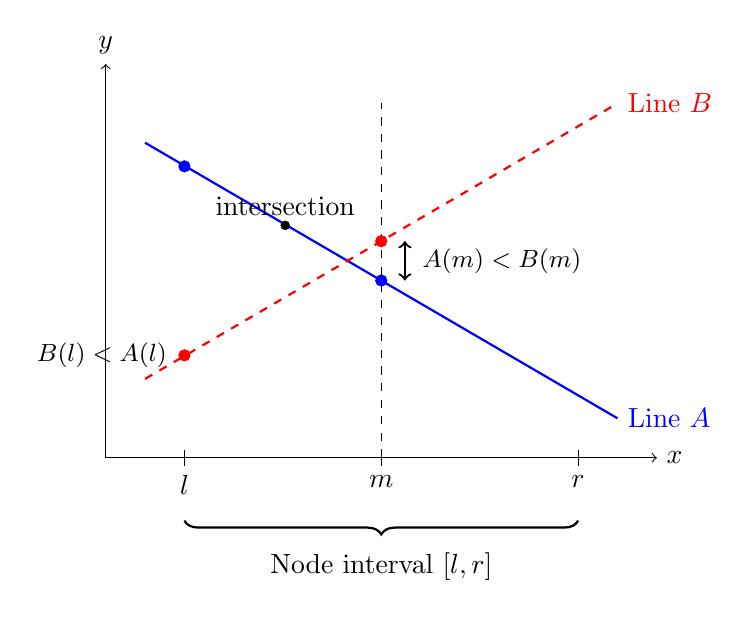
\begin{tikzpicture}[scale=1.0]
\draw[->] (0,0) -- (7,0) node[right] {$x$};
\draw[->] (0,0) -- (0,5) node[above] {$y$};
\draw (1,0.1) -- (1,-0.1) node[below] {$l$};
\draw (6,0.1) -- (6,-0.1) node[below] {$r$};
\draw (3.5,0.1) -- (3.5,-0.1) node[below] {$m$};
\draw[thick, blue] (0.5,4.0) -- (6.5,0.5) node[right] {Line $A$};
\draw[thick, red, dashed] (0.5,1.0) -- (6.5,4.5) node[right] {Line $B$};
\filldraw[black] (2.28,2.95) circle (1.5pt) node[above] {intersection};
\draw[dashed] (3.5,0) -- (3.5,4.5);
\filldraw[blue] (3.5,2.25) circle (2pt);
\filldraw[red] (3.5,2.75) circle (2pt);
\draw[thick, <->] (3.8,2.25) -- (3.8,2.75);
\node[right] at (3.9,2.5) {\small $A(m) < B(m)$};
\filldraw[blue] (1,3.7) circle (2pt);
\filldraw[red] (1,1.3) circle (2pt);
\node[left] at (0.9,1.3) {\small $B(l) < A(l)$};
\draw[thick, decorate, decoration={brace, amplitude=5pt, mirror}] (1,-0.8) -- (6,-0.8) node[midway, below=8pt] {Node interval $[l, r]$};
\end{tikzpicture}
\caption{Interval Advantage Line Diagram. The node stores Line $A$ because it achieves the lower value at the midpoint. Line $B$ is routed to the left child where it may be optimal.}
\label{fig:interval-advantage}
\end{figure}

\paragraph{Insertion.} To insert a new line, we compare it with the line already stored at the current node. The line that is lower at the midpoint is kept at the node, and the "losing" line is routed to a child interval where it might potentially be optimal.

\begin{algorithm}[H]
\caption{LICT Line Insertion}
\label{alg:insert}
\begin{algorithmic}[1]
\Require Node pointer $node$, new line $new\_line$, interval $[l, r]$
\If{$node$ is null}
\State $node \gets \text{new Node}(new\_line)$
\State \Return
\EndIf
\State $m \gets l + (r - l) / 2$
\State $lef \gets new\_line.eval(l) < node.line.eval(l)$
\State $midf \gets new\_line.eval(m) < node.line.eval(m)$
\If{$midf$}
\State swap($node.line$, $new\_line$)
\EndIf
\If{$r - l < \epsilon$} \Comment{Max depth reached; drop the losing line}
\State \Return
\EndIf
\If{$lef \neq midf$}
\State \Call{Insert}{$node.left$, $new\_line$, $l$, $m$}
\Else
\State \Call{Insert}{$node.right$, $new\_line$, $m$, $r$}
\EndIf
\end{algorithmic}
\end{algorithm}

We illustrate the insertion process with a concrete example. Consider the following lines:
\begin{itemize}
    \item $f_0(x) = x$
    \item $f_1(x) = 2x - 4$
    \item $f_2(x) = 0.5x + 2$
    \item $f_{new}(x) = -x + 10$
\end{itemize}

Figure~\ref{fig:insertion-example-before} shows the tree before inserting $f_{new}$. Figure~\ref{fig:insertion-example-after} shows the tree after insertion, demonstrating how $f_{new}$ displaces an existing line.

\begin{figure}[H]
\centering
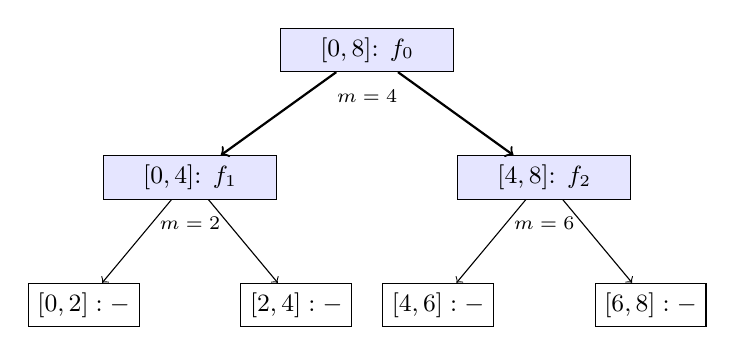
\begin{tikzpicture}[scale=0.9, every node/.style={font=\small}]
\node[draw, rectangle, fill=blue!10, minimum width=2.2cm] (root) at (0,0) {$[0, 8]$: $f_0$};
\node[below=0.1cm of root] {\scriptsize $m=4$};
\node[draw, rectangle, fill=blue!10, minimum width=2.2cm] (l1) at (-2.5,-1.8) {$[0, 4]$: $f_1$};
\node[below=0.1cm of l1] {\scriptsize $m=2$};
\node[draw, rectangle, fill=blue!10, minimum width=2.2cm] (r1) at (2.5,-1.8) {$[4, 8]$: $f_2$};
\node[below=0.1cm of r1] {\scriptsize $m=6$};
\node[draw, rectangle, minimum width=1.4cm] (l2l) at (-4.0,-3.6) {$[0, 2]: -$};
\node[draw, rectangle, minimum width=1.4cm] (l2r) at (-1.0,-3.6) {$[2, 4]: -$};
\node[draw, rectangle, minimum width=1.4cm] (r2l) at (1.0,-3.6) {$[4, 6]: -$};
\node[draw, rectangle, minimum width=1.4cm] (r2r) at (4.0,-3.6) {$[6, 8]: -$};
\draw[->, thick] (root) -- (l1); \draw[->, thick] (root) -- (r1);
\draw[->] (l1) -- (l2l); \draw[->] (l1) -- (l2r);
\draw[->] (r1) -- (r2l); \draw[->] (r1) -- (r2r);
\end{tikzpicture}
\caption{Tree structure before inserting $f_{new}(x) = -x + 10$. Currently stores $f_0(x)=x$ at root, $f_1(x)=2x-4$ at $[0,4]$, and $f_2(x)=0.5x+2$ at $[4,8]$.}
\label{fig:insertion-example-before}
\end{figure}

\textbf{Why the lines are positioned there:}
\begin{itemize}
    \item $f_1$ at $[0,4]$: At root $[0,8]$ with $m=4$, $f_0(4)=4$ and $f_1(4)=4$ (equal). Since $f_1(0)=-4 < f_0(0)=0$, $f_1$ is routed to the left child $[0,4]$ where it gets stored.
    \item $f_2$ at $[4,8]$: Similarly, $f_2(4)=4$ equals $f_0(4)$, and since $f_2(8)=6 > f_0(8)=8$... wait, that's wrong. Let me reconsider.
\end{itemize}

Actually, let me trace more carefully. For $f_2(x)=0.5x+2$:
- At root $[0,8]$, $m=4$: $f_0(4)=4$, $f_2(4)=4$ (equal)
- At left endpoint $x=0$: $f_0(0)=0$, $f_2(0)=2$, so $f_0(0) < f_2(0)$
- At right endpoint $x=8$: $f_0(8)=8$, $f_2(8)=6$, so $f_2(8) < f_0(8)$

Since $f_0$ is lower at $m=4$ and $f_2$ is lower at $x=8$ (right side), $f_0$ stays at root and $f_2$ is routed to the right child $[4,8]$.

\begin{figure}[H]
\centering
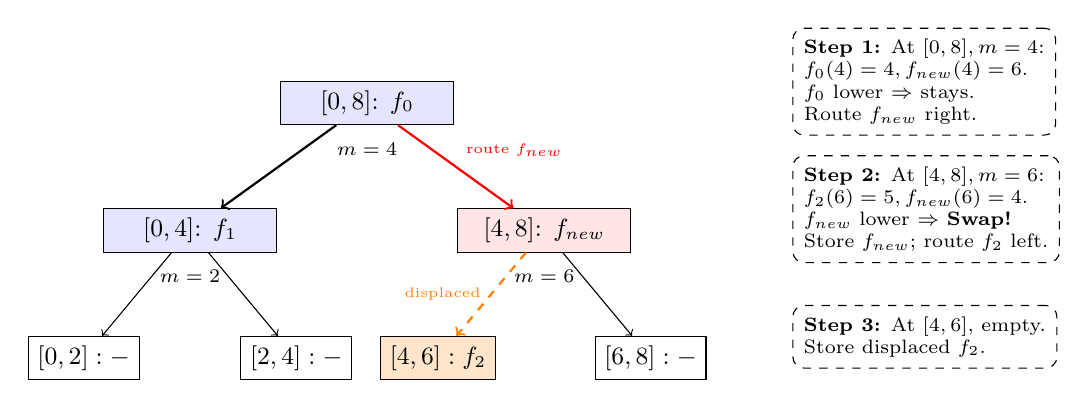
\begin{tikzpicture}[scale=0.9, every node/.style={font=\small}]
\node[draw, rectangle, fill=blue!10, minimum width=2.2cm] (root) at (0,0) {$[0, 8]$: $f_0$};
\node[below=0.1cm of root] {\scriptsize $m=4$};
\node[draw, rectangle, fill=blue!10, minimum width=2.2cm] (l1) at (-2.5,-1.8) {$[0, 4]$: $f_1$};
\node[below=0.1cm of l1] {\scriptsize $m=2$};
\node[draw, rectangle, fill=red!10, minimum width=2.2cm] (r1) at (2.5,-1.8) {$[4, 8]$: $f_{new}$};
\node[below=0.1cm of r1] {\scriptsize $m=6$};
\node[draw, rectangle, minimum width=1.4cm] (l2l) at (-4.0,-3.6) {$[0, 2]: -$};
\node[draw, rectangle, minimum width=1.4cm] (l2r) at (-1.0,-3.6) {$[2, 4]: -$};
\node[draw, rectangle, fill=orange!20, minimum width=1.4cm] (r2l) at (1.0,-3.6) {$[4, 6]: f_2$};
\node[draw, rectangle, minimum width=1.4cm] (r2r) at (4.0,-3.6) {$[6, 8]: -$};
\draw[->, thick] (root) -- (l1);
\draw[->, thick, red] (root) -- (r1) node[midway, above right, font=\tiny] {route $f_{new}$};
\draw[->] (l1) -- (l2l); \draw[->] (l1) -- (l2r);
\draw[->, thick, dashed, orange] (r1) -- (r2l) node[midway, left, font=\tiny] {displaced};
\draw[->] (r1) -- (r2r);

\begin{scope}[xshift=6.0cm]
\node[draw, dashed, rounded corners, inner sep=4pt, align=left, anchor=west, fill=white, font=\scriptsize] at (0, 0.3) {
\textbf{Step 1:} At $[0,8], m=4$:\\
$f_0(4)=4, f_{new}(4)=6$.\\
$f_0$ lower $\Rightarrow$ stays.\\
Route $f_{new}$ right.
};
\node[draw, dashed, rounded corners, inner sep=4pt, align=left, anchor=west, fill=white, font=\scriptsize] at (0, -1.5) {
\textbf{Step 2:} At $[4,8], m=6$:\\
$f_2(6)=5, f_{new}(6)=4$.\\
$f_{new}$ lower $\Rightarrow$ \textbf{Swap!}\\
Store $f_{new}$; route $f_2$ left.
};
\node[draw, dashed, rounded corners, inner sep=4pt, align=left, anchor=west, fill=white, font=\scriptsize] at (0, -3.3) {
\textbf{Step 3:} At $[4,6]$, empty.\\
Store displaced $f_2$.
};
\end{scope}
\end{tikzpicture}
\caption{Tree structure after inserting $f_{new}(x) = -x + 10$. At $[4,8]$, $f_{new}(6)=4 < f_2(6)=5$, so $f_{new}$ swaps in and $f_2$ is displaced to $[4,6]$.}
\label{fig:insertion-example-after}
\end{figure}

\paragraph{Query.} We traverse the path to $x_0$, evaluating all stored lines along the path. The minimum value encountered equals the lower envelope at $x_0$ because any line that could be optimal at $x_0$ is stored on this path.

\begin{algorithm}[H]
\caption{LICT Query}
\label{alg:query}
\begin{algorithmic}[1]
\Require Node pointer $node$, query coordinate $x$, interval $[l, r]$
\Ensure Minimum value at coordinate $x$
\If{$node$ is null}
\State \Return $+\infty$
\EndIf
\State $m \gets l + (r - l) / 2$
\State $val \gets node.line.eval(x)$
\If{$r - l < \epsilon$}
\State \Return $val$
\EndIf
\If{$x \leq m$}
\State \Return $\min(val, \text{\Call{Query}{$node.left$, $x$, $l$, $m$}})$
\Else
\State \Return $\min(val, \text{\Call{Query}{$node.right$, $x$, $m$, $r$}})$
\EndIf
\end{algorithmic}
\end{algorithm}

\subsection{Complexity Analysis}

\textbf{Time Complexity:} Both insertion and query operations traverse a single root-to-leaf path of length $O(\log C)$, performing $O(1)$ work per node. Total time is $O(\log C)$.

\textbf{Space Complexity:} Each insertion creates at most one new node per level. With $n$ insertions, total space is $O(n \log C)$.

\textbf{Deletion:} The standard LICT does not support efficient deletion. Removing a line would require traversing all nodes where that line might be stored, which requires $\Omega(n)$ time in the worst case.

\section{Conclusion}
The Li-Chao tree provides a robust and efficient alternative for dynamic line envelope maintenance. Its numerical stability and ease of implementation make it a preferred choice in many practical scenarios, especially under the time constraints of algorithmic competitions.

\end{document}
